\documentclass[12pt]{article}

\usepackage{amsmath}
\usepackage{amssymb}
\usepackage{amsfonts}
\usepackage{geometry}
\usepackage{fancyhdr}
\usepackage{tikz}
\usetikzlibrary{matrix}

% Page setup
\geometry{margin=1in}
\setlength{\headheight}{15pt}
\pagestyle{fancy}
\fancyhf{}
\fancyhead[L]{Integrated Algebra 2 and Precalculus}
\fancyhead[R]{Assignment: Chapter 9 of Algebra 2}
\fancyfoot[C]{Page \thepage}

\begin{document}

\begin{center}
\textbf{\Large Systems of Linear Equations: From Two Variables to Matrices} \\
\vspace{0.5cm}
\makebox[0.4\textwidth]{Name: \enspace\hrulefill}
\hspace{0.1\textwidth}
\makebox[0.4\textwidth]{Date: \enspace\hrulefill}
\end{center}

\vspace{0.5cm}

\section{Introduction}

Systems of linear equations appear everywhere in mathematics, science, engineering, and economics. From finding the intersection of lines to modeling complex networks, these systems provide a powerful framework for solving real-world problems.

In this chapter, we'll explore systems with two, three, and more variables, discovering how the geometric interpretation changes as we move from lines in a plane to planes in three-dimensional space. We'll also introduce the elegant mathematical framework of matrices and linear algebra that makes solving large systems both systematic and efficient.

\section{Systems of Two Linear Equations}

\subsection{Fundamental Concepts}

A \textbf{system of linear equations} is a collection of linear equations involving the same set of variables. A \textbf{solution} to the system is a set of values for the variables that satisfies all equations simultaneously.

For two variables $x$ and $y$, a general system has the form:
\begin{align}
a_1x + b_1y &= c_1 \\
a_2x + b_2y &= c_2
\end{align}

\subsection{Geometric Interpretation}

Each linear equation represents a line in the $xy$-plane. The solution to the system corresponds to the intersection point(s) of these lines:

\begin{itemize}
\item \textbf{Unique solution:} The lines intersect at exactly one point
\item \textbf{No solution:} The lines are parallel (but not identical)  
\item \textbf{Infinitely many solutions:} The lines are identical (coincident)
\end{itemize}

\subsection{Solution Methods}

\textbf{Method 1: Substitution}
\begin{enumerate}
\item Solve one equation for one variable in terms of the other
\item Substitute this expression into the second equation
\item Solve for the remaining variable
\item Back-substitute to find the other variable
\end{enumerate}

\textbf{Method 2: Elimination}
\begin{enumerate}
\item Multiply equations by constants to make coefficients of one variable equal (or opposite)
\item Add or subtract equations to eliminate that variable
\item Solve for the remaining variable
\item Back-substitute to find the other variable
\end{enumerate}

\textbf{Example:} Solve the system
\begin{align}
2x + 3y &= 7 \\
x - y &= 1
\end{align}

\textbf{Solution by elimination:}
From the second equation: $x = y + 1$

Substituting into the first equation:
$2(y + 1) + 3y = 7$
$2y + 2 + 3y = 7$
$5y = 5$
$y = 1$

Therefore: $x = 1 + 1 = 2$

The solution is $(x, y) = (2, 1)$.

\section{Systems of Three Linear Equations}

\subsection{Three Variables, Three Equations}

A system of three linear equations in three variables has the general form:
\begin{align}
a_1x + b_1y + c_1z &= d_1 \\
a_2x + b_2y + c_2z &= d_2 \\
a_3x + b_3y + c_3z &= d_3
\end{align}

\subsection{Geometric Interpretation in Three Dimensions}

Each equation represents a \textbf{plane} in three-dimensional space. The solution set corresponds to the intersection of these three planes:

\begin{itemize}
\item \textbf{Unique solution:} The three planes intersect at a single point
\item \textbf{No solution:} The planes have no common intersection (e.g., three parallel planes)
\item \textbf{Infinitely many solutions:} The planes intersect along a line or are identical
\end{itemize}

\subsection{Gaussian Elimination}

For larger systems, we use \textbf{Gaussian elimination}, a systematic method that transforms the system into an equivalent but simpler form.

\textbf{Goal:} Transform the system into \textbf{row echelon form}, where:
\begin{itemize}
\item All nonzero rows are above any rows of all zeros
\item The leading coefficient (pivot) of each row is to the right of the leading coefficient of the row above it
\item All entries in a column below a pivot are zeros
\end{itemize}

\textbf{Elementary Row Operations:}
\begin{enumerate}
\item Multiply a row by a nonzero constant
\item Add a multiple of one row to another row
\item Interchange two rows
\end{enumerate}

\textbf{Example:} Solve the system
\begin{align}
x + 2y + z &= 6 \\
2x - y + 3z &= 14 \\
x + y - z &= -2
\end{align}

\textbf{Step 1:} Write the augmented matrix
$$\left[\begin{array}{ccc|c}
1 & 2 & 1 & 6 \\
2 & -1 & 3 & 14 \\
1 & 1 & -1 & -2
\end{array}\right]$$

\textbf{Step 2:} Use row operations to get zeros below the first pivot
$R_2 \leftarrow R_2 - 2R_1$: 
$$\left[\begin{array}{ccc|c}
1 & 2 & 1 & 6 \\
0 & -5 & 1 & 2 \\
1 & 1 & -1 & -2
\end{array}\right]$$

$R_3 \leftarrow R_3 - R_1$:
$$\left[\begin{array}{ccc|c}
1 & 2 & 1 & 6 \\
0 & -5 & 1 & 2 \\
0 & -1 & -2 & -8
\end{array}\right]$$

\textbf{Step 3:} Get zeros below the second pivot
$R_3 \leftarrow R_3 - \frac{1}{5}R_2$:
$$\left[\begin{array}{ccc|c}
1 & 2 & 1 & 6 \\
0 & -5 & 1 & 2 \\
0 & 0 & -\frac{11}{5} & -\frac{42}{5}
\end{array}\right]$$

\textbf{Step 4:} Back-substitution
From the third row: $-\frac{11}{5}z = -\frac{42}{5}$, so $z = \frac{42}{11}$

From the second row: $-5y + z = 2$, so $y = \frac{z - 2}{5} = \frac{\frac{42}{11} - 2}{5} = \frac{20}{55} = \frac{4}{11}$

From the first row: $x + 2y + z = 6$, so $x = 6 - 2y - z = 6 - 2 \cdot \frac{4}{11} - \frac{42}{11} = \frac{16}{11}$

The solution is $\left(\frac{16}{11}, \frac{4}{11}, \frac{42}{11}\right)$.

\section{Introduction to Matrices}

\subsection{Matrix Notation}

A \textbf{matrix} is a rectangular array of numbers. For a system of linear equations, we can represent it using matrices:

\textbf{Coefficient Matrix} $A$:
$$A = \begin{pmatrix}
a_1 & b_1 & c_1 \\
a_2 & b_2 & c_2 \\
a_3 & b_3 & c_3
\end{pmatrix}$$

\textbf{Variable Vector} $\mathbf{x}$:
$$\mathbf{x} = \begin{pmatrix} x \\ y \\ z \end{pmatrix}$$

\textbf{Constant Vector} $\mathbf{b}$:
$$\mathbf{b} = \begin{pmatrix} d_1 \\ d_2 \\ d_3 \end{pmatrix}$$

The system can be written compactly as: $A\mathbf{x} = \mathbf{b}$

\subsection{Matrix Operations}

\textbf{Matrix Addition:} Add corresponding entries
$$\begin{pmatrix} a & b \\ c & d \end{pmatrix} + \begin{pmatrix} e & f \\ g & h \end{pmatrix} = \begin{pmatrix} a+e & b+f \\ c+g & d+h \end{pmatrix}$$

\textbf{Scalar Multiplication:} Multiply every entry by the scalar
$$k \begin{pmatrix} a & b \\ c & d \end{pmatrix} = \begin{pmatrix} ka & kb \\ kc & kd \end{pmatrix}$$

\textbf{Matrix Multiplication:} For compatible matrices $A$ and $B$, the $(i,j)$ entry of $AB$ is the dot product of the $i$-th row of $A$ with the $j$-th column of $B$.

$$\begin{pmatrix} a & b \\ c & d \end{pmatrix} \begin{pmatrix} e & f \\ g & h \end{pmatrix} = \begin{pmatrix} ae+bg & af+bh \\ ce+dg & cf+dh \end{pmatrix}$$

\subsection{Determinants and Invertibility}

For a $2 \times 2$ matrix $A = \begin{pmatrix} a & b \\ c & d \end{pmatrix}$, the \textbf{determinant} is:
$$\det(A) = ad - bc$$

If $\det(A) \neq 0$, then $A$ is \textbf{invertible} and the system $A\mathbf{x} = \mathbf{b}$ has a unique solution:
$$\mathbf{x} = A^{-1}\mathbf{b}$$

where $A^{-1} = \frac{1}{\det(A)} \begin{pmatrix} d & -b \\ -c & a \end{pmatrix}$

\newpage

\section{Practice Problems}

\textbf{Part A: Two-Variable Systems}

\textbf{1.} Solve the following systems using both substitution and elimination methods:

\begin{enumerate}
\item[(a)] $\begin{cases} 3x + 2y = 12 \\ x - y = 1 \end{cases}$
\vspace{3cm}

\item[(b)] $\begin{cases} 2x + 5y = 16 \\ 3x - 2y = -3 \end{cases}$
\vspace{3cm}

\item[(c)] $\begin{cases} 4x - 6y = 8 \\ -2x + 3y = -4 \end{cases}$
\vspace{3cm}
\end{enumerate}

\textbf{2.} For each system in Problem 1, describe the geometric relationship between the two lines (intersecting, parallel, or coincident).
\vspace{2cm}

\textbf{3.} A theater sells adult tickets for \$15 and student tickets for \$8. One evening, they sold 240 total tickets and collected \$2,940 in revenue. How many adult and student tickets were sold?
\vspace{4cm}

\newpage

\textbf{Part B: Three-Variable Systems}

\textbf{4.} Solve the following systems using Gaussian elimination:

\begin{enumerate}
\item[(a)] $\begin{cases} 
x + y + z = 6 \\
2x - y + 3z = 14 \\
x + 2y - z = 0
\end{cases}$
\vspace{5cm}

\item[(b)] $\begin{cases}
2x + 3y - z = 1 \\
x - y + 2z = 4 \\
3x + y + z = 7
\end{cases}$
\vspace{5cm}
\end{enumerate}

\textbf{5.} A company produces three products: A, B, and C. The production requirements are:
\begin{itemize}
\item Product A requires 2 hours of labor, 1 hour of machine time, and \$3 of materials
\item Product B requires 1 hour of labor, 2 hours of machine time, and \$4 of materials  
\item Product C requires 3 hours of labor, 1 hour of machine time, and \$2 of materials
\end{itemize}

If the company has 100 hours of labor, 80 hours of machine time, and \$200 for materials available, how many of each product should they produce to use all resources exactly?
\vspace{6cm}

\newpage

\textbf{Part C: Matrix Operations}

\textbf{6.} Given matrices $A = \begin{pmatrix} 2 & -1 \\ 3 & 4 \end{pmatrix}$, $B = \begin{pmatrix} 1 & 2 \\ -1 & 3 \end{pmatrix}$, and $C = \begin{pmatrix} 5 \\ -2 \end{pmatrix}$, compute:

\begin{enumerate}
\item[(a)] $A + B$
\vspace{2cm}

\item[(b)] $AB$
\vspace{3cm}

\item[(c)] $AC$
\vspace{3cm}

\item[(d)] $\det(A)$ and $\det(B)$
\vspace{2cm}
\end{enumerate}

\textbf{7.} Write the following system in matrix form $A\mathbf{x} = \mathbf{b}$ and solve using the matrix inverse method:

$$\begin{cases}
2x + 3y = 7 \\
x - y = 1
\end{cases}$$
\vspace{4cm}

\textbf{8.} For what value(s) of $k$ does the following system have:
\begin{enumerate}
\item[(a)] A unique solution?
\item[(b)] No solution?
\item[(c)] Infinitely many solutions?
\end{enumerate}

$$\begin{cases}
x + 2y = 3 \\
2x + ky = 6
\end{cases}$$
\vspace{4cm}

\newpage

\textbf{Part D: Challenge Problems}

\textbf{9.} (Parametric Solutions) Consider the system:
$$\begin{cases}
x + 2y - z = 1 \\
2x + 4y - 2z = 2
\end{cases}$$

\begin{enumerate}
\item[(a)] Show that this system has infinitely many solutions.
\vspace{3cm}

\item[(b)] Express the general solution in parametric form using a parameter $t$.
\vspace{3cm}

\item[(c)] Find three specific solutions to the system.
\vspace{2cm}
\end{enumerate}

\textbf{10.} (Network Flow) A city's traffic network has four intersections connected by one-way streets. The flow rates (cars per hour) must satisfy the constraint that flow in equals flow out at each intersection.

\begin{center}
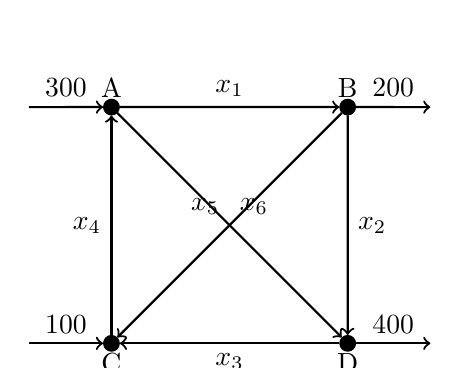
\begin{tikzpicture}[scale=1.5]
    % Intersections
    \node[circle,draw,fill=black,inner sep=2pt] (A) at (0,2) {};
    \node[circle,draw,fill=black,inner sep=2pt] (B) at (2,2) {};
    \node[circle,draw,fill=black,inner sep=2pt] (C) at (0,0) {};
    \node[circle,draw,fill=black,inner sep=2pt] (D) at (2,0) {};
    
    % Labels
    \node[above] at (A) {A};
    \node[above] at (B) {B};
    \node[below] at (C) {C};
    \node[below] at (D) {D};
    
    % Arrows with flow variables
    \draw[->,thick] (A) -- (B) node[midway,above] {$x_1$};
    \draw[->,thick] (B) -- (D) node[midway,right] {$x_2$};
    \draw[->,thick] (D) -- (C) node[midway,below] {$x_3$};
    \draw[->,thick] (C) -- (A) node[midway,left] {$x_4$};
    \draw[->,thick] (A) -- (D) node[midway,above left] {$x_5$};
    \draw[->,thick] (B) -- (C) node[midway,above right] {$x_6$};
    
    % External flows
    \draw[->,thick] (-0.7,2) -- (A) node[midway,above] {300};
    \draw[->,thick] (B) -- (2.7,2) node[midway,above] {200};
    \draw[->,thick] (-0.7,0) -- (C) node[midway,above] {100};
    \draw[->,thick] (D) -- (2.7,0) node[midway,above] {400};
\end{tikzpicture}
\end{center}

If 300 cars/hour enter at A, 200 cars/hour exit at B, 100 cars/hour enter at C, and 400 cars/hour exit at D, set up and solve the system of equations for the internal flow rates $x_1, x_2, x_3, x_4, x_5, x_6$.
\vspace{6cm}

\textbf{11.} (Linear Algebra Connection) Research and explain in your own words:
\begin{enumerate}
\item[(a)] What is the relationship between the number of solutions to a system and the rank of its coefficient matrix?
\vspace{3cm}

\item[(b)] How does the concept of linear independence relate to systems of equations?
\vspace{3cm}

\item[(c)] Why is Gaussian elimination considered a fundamental algorithm in linear algebra?
\vspace{3cm}
\end{enumerate}

\end{document}